
\section{parameters.xml}

The parameter file contains density constraints for the RBA model,
user-defined parameters and functions.


\subsection{RBAParameters}
\label{sec:rba_parameters}

The outermost portion of the parameter file is an instance of class
\rbaparameters, shown in Figure~\ref{fig:parameters_doc}.

\begin{figure}
  \centering
  \includegraphics[scale=0.8]{figures/parameters_doc}
  \caption{XML structure of parameter document.}
\label{fig:parameters_doc}
\end{figure}

\rbaparameters{} has no simple attributes.
It includes exactly one instance of \textbf{ListOf} container classes.
All \textbf{ListOf} classes do not have own attributes,
they are merely used to organize a list of instances from another class.


\subsection{TargetDensity}
\label{sec:target_density}

The \targetdensity{} class is used to define density constraints
(Fig.~\ref{fig:parameters_target_density}).
In a RBA model, a density constraint defines how many molecules
a given compartment can contain.
It inherits \targetvalue{} for the constraint definition part.

\begin{figure}
  \centering
  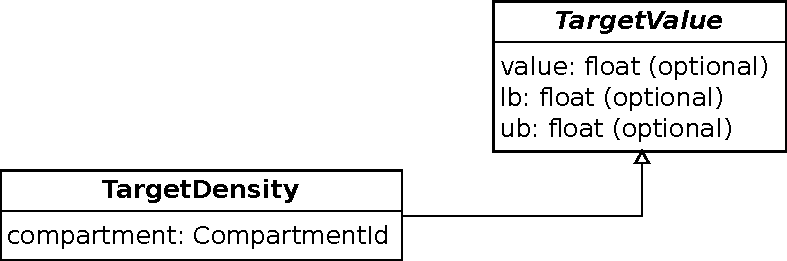
\includegraphics[scale=0.8]{figures/parameters_target_density}
  \caption{Class used to store density constraints.}
\label{fig:parameters_target_density}
\end{figure}

\paragraph{The \textit{compartment} attribute}
The \textbf{compartment} attribute must match the identifier of a \compartment.


\subsection{TargetValue}
\label{sec:target_value}

The \targetvalue{} class is used to define the sign of an additional RBA
constraint and the value of its second member
(Fig.~\ref{fig:parameters_target_density}).
It is designed to be inherited.
The child class usually holds information about the first member of the
constraint
(\textit{e.g.} compartment for a density constraint,
metabolite for a production constraint).

\paragraph{The \textit{value}, \textit{lb} and \textit{ub} attributes}
Every attribute can be left undefined, set to a real number or
contain the identifier of a \function{} or an \aggregate.
In the latter case, its value will be growth-rate dependent.

If \textbf{value} is defined, the constraint is an equally constraint.
\textbf{lb} and \textbf{ub} are ignored.
If \textbf{value} is undefined, \textbf{lb} (resp. \textbf{ub}) defines
a lower bound (resp.\ upper bound) inequality constraint.
Note that \textbf{lb} and \textbf{ub} may both be defined, yielding two
separate inequality constraints.

\subsection{Function}
\label{sec:function}

The \function{} class is used for user-defined functions and parameters
(Fig.~\ref{fig:parameters_function}).
Implictly, all functions defined here are functions of \emph{growth rate}.
Every function holds a \textbf{ListOfParameters},
where \parameter{} are defined according to each type of function.

\begin{figure}
  \centering
  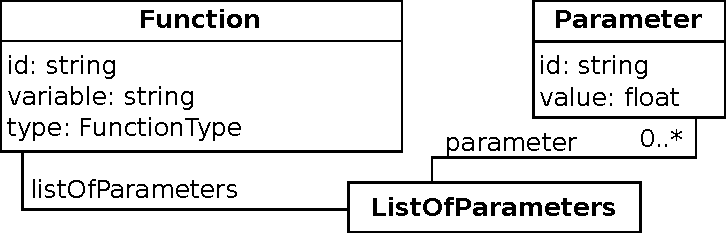
\includegraphics[scale=0.8]{figures/parameters_function}
  \caption{Class used to store user-defined functions.}
\label{fig:parameters_function}
\end{figure}

\paragraph{The \textit{id} attribute}
The \textbf{id} attribute is a string defining the identifier of the function.

\paragraph{The \textit{type} attribute}
The \textbf{type} attribute is a string that must match a known function type.
Currently, the supported types are:
\begin{itemize}
  \item \textbf{constant}.
  Constant function with parameter
  \textit{CONSTANT}.
  \item \textbf{linear}.
  Linear function with parameters
  \textit{LINEAR\_CONSTANT}, \textit{LINEAR\_COEF},
  \textit{X\_MIN}, \textit{X\_MAX}, \textit{Y\_MIN}, \textit{Y\_MAX}.
  The 4 last parameters are used to saturate the function.
  If the variable (growth rate) is outside of the [X\_MIN,~X\_MAX] range,
  it is set to the closest value in that range.
  The same applies for the return value and the [Y\_MIN,~Y\_MAX] range.
  \item \textbf{exponential}.
  Exponential function with parameter \textit{RATE}.
  \item \textbf{indicator}.
  Indicator function with parameters
  \textit{X\_MIN} and \textit{X\_MAX}.
  This function returns one if the variable (growth rate) is in the
  [X\_MIN,~X\_MAX], zero otherwise.
  \item \textbf{michaelisMenten}.
  Michaelis Menten function with parameters
  \textit{kmax}, \textit{Km} and \textit{Y\_MIN} (optional).
  If Y\_MIN is defined, any return value lower than Y\_MIN will be set to
  Y\_MIN.\@
\end{itemize}


\subsection{Parameter}
\label{sec:parameter}

The \parameter{} class is used to store the values of function parameters
(Fig.~\ref{fig:parameters_function}).

\paragraph{The \textit{id} attribute}
The \textbf{id} attribute is a string that should match a valid parameter
identifier.
The list of valid parameters for each type of \function{} is listed above.

\paragraph{The \textit{value} attribute}
The \textbf{value} attribute is a real number representing
the value of the attribute.


\subsection{Aggregate}
\label{sec:aggregate}

The \aggregate{} class is used to assemble user-defined functions
(Fig.~\ref{fig:parameters_aggregate}).
Every aggregate holds a \textbf{ListOfFunctionReferences},
where each \functionreference{} refers to a previously defined function.

\begin{figure}
  \centering
  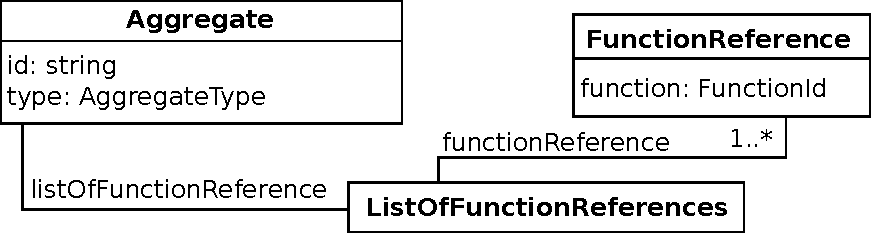
\includegraphics[scale=0.8]{figures/parameters_aggregate}
  \caption{Class used to store user-defined aggregates.}
\label{fig:parameters_aggregate}
\end{figure}

\paragraph{The \textit{id} attribute}
The \textbf{id} attribute is a string defining the identifier of the aggregate.

\paragraph{The \textit{type} attribute}
The \textbf{type} attribute is a string that must match a known aggregate type.
Currently, the supported types are:
\begin{itemize}
  \item \textbf{multiplication}.
  The result is the multiplication of the values returned by the function
  listed in the aggregate at current growth rate.
\end{itemize}


\subsection{FunctionReference}
\label{sec:function_reference}

The \functionreference{} class is used to refer to a user-defined \function{}
(Fig.~\ref{fig:parameters_aggregate}).

\paragraph{The \textit{function} attribute}
The \textbf{function} attribute is a string that must match the identifier
of a user-defined \function{}.
